\addcontentsline{toc}{section}{Appendix}
\section*{Appendix}
\addcontentsline{toc}{subsection}{Design Documents}
\subsection*{Design documents}
%Put CAD drawings, additional sketches.  If there are many, it is better to put the high-level drawings (assemblies), then put the rest of the drawings somewhere that the reader can retreive them (SVN, etc.).  Don't forget to put a link here.

\begin{figure}[H]
\centering
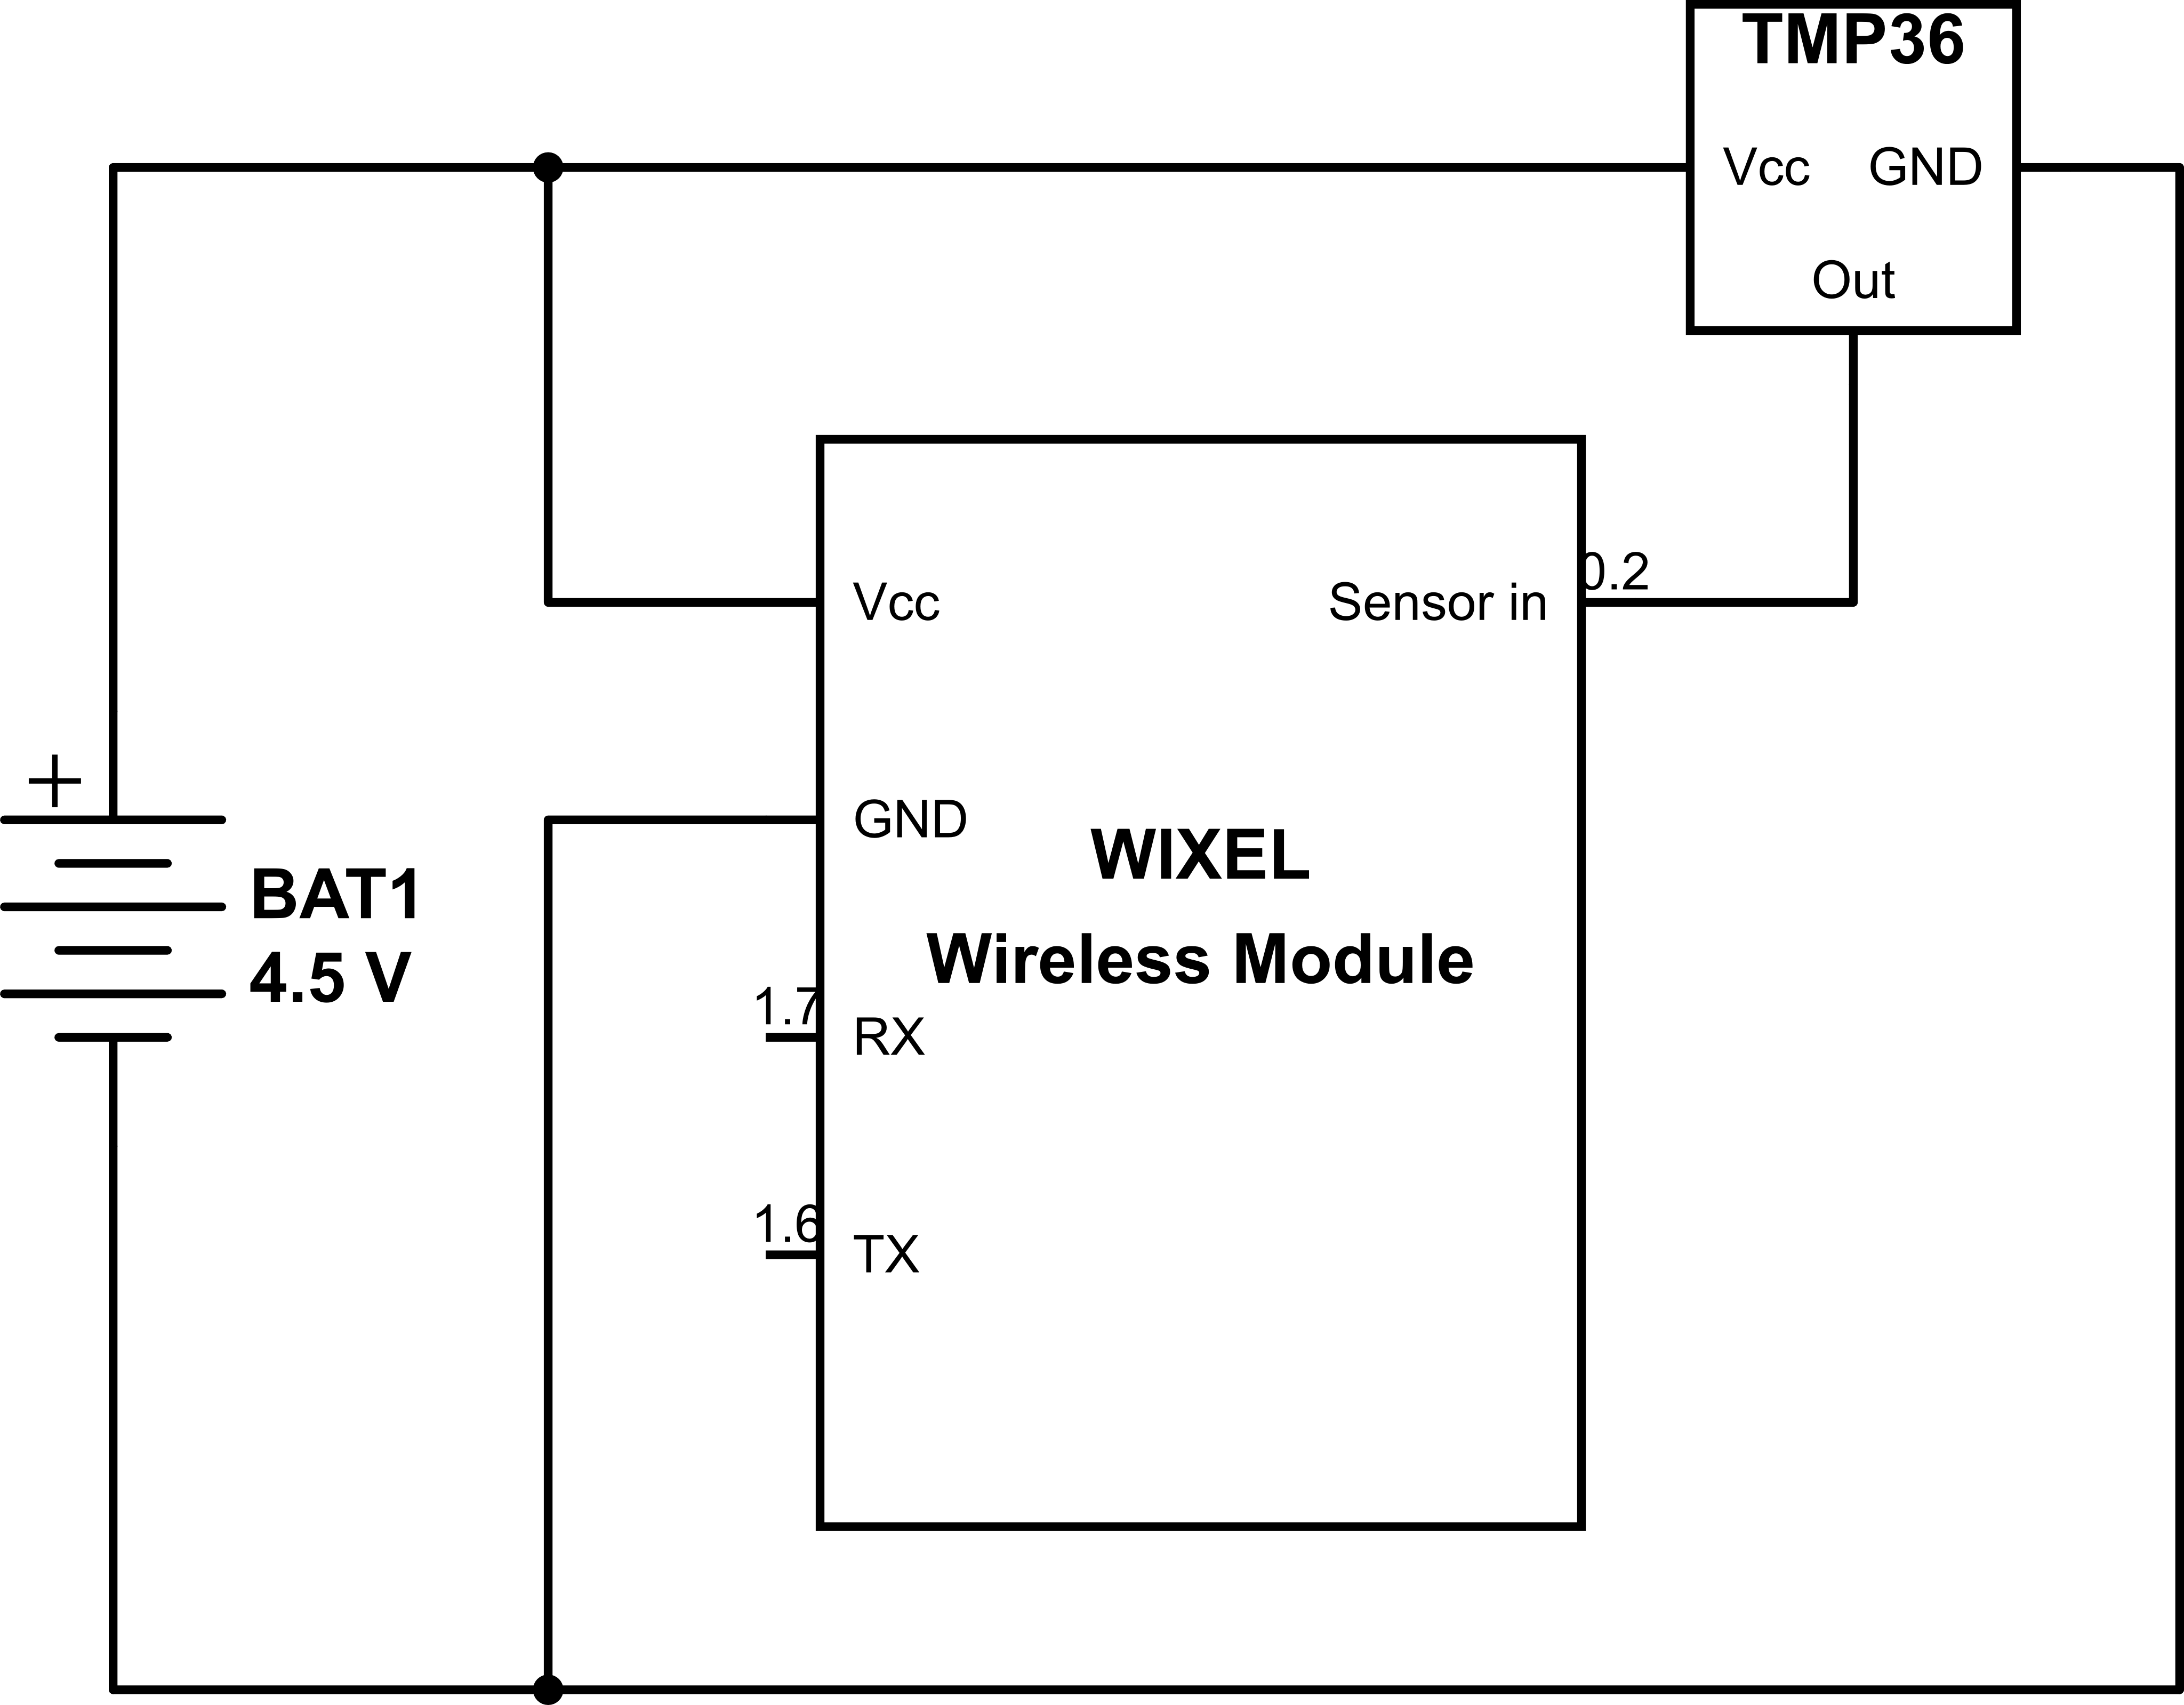
\includegraphics[width=0.5\linewidth]{graphics/sensormodule_schematic}
\caption{Electrical Schematic Diagram of the Wireless Sensor Module\label{fig:sensormodule_schematic}}
\end{figure}

\begin{figure}[H]
\centering
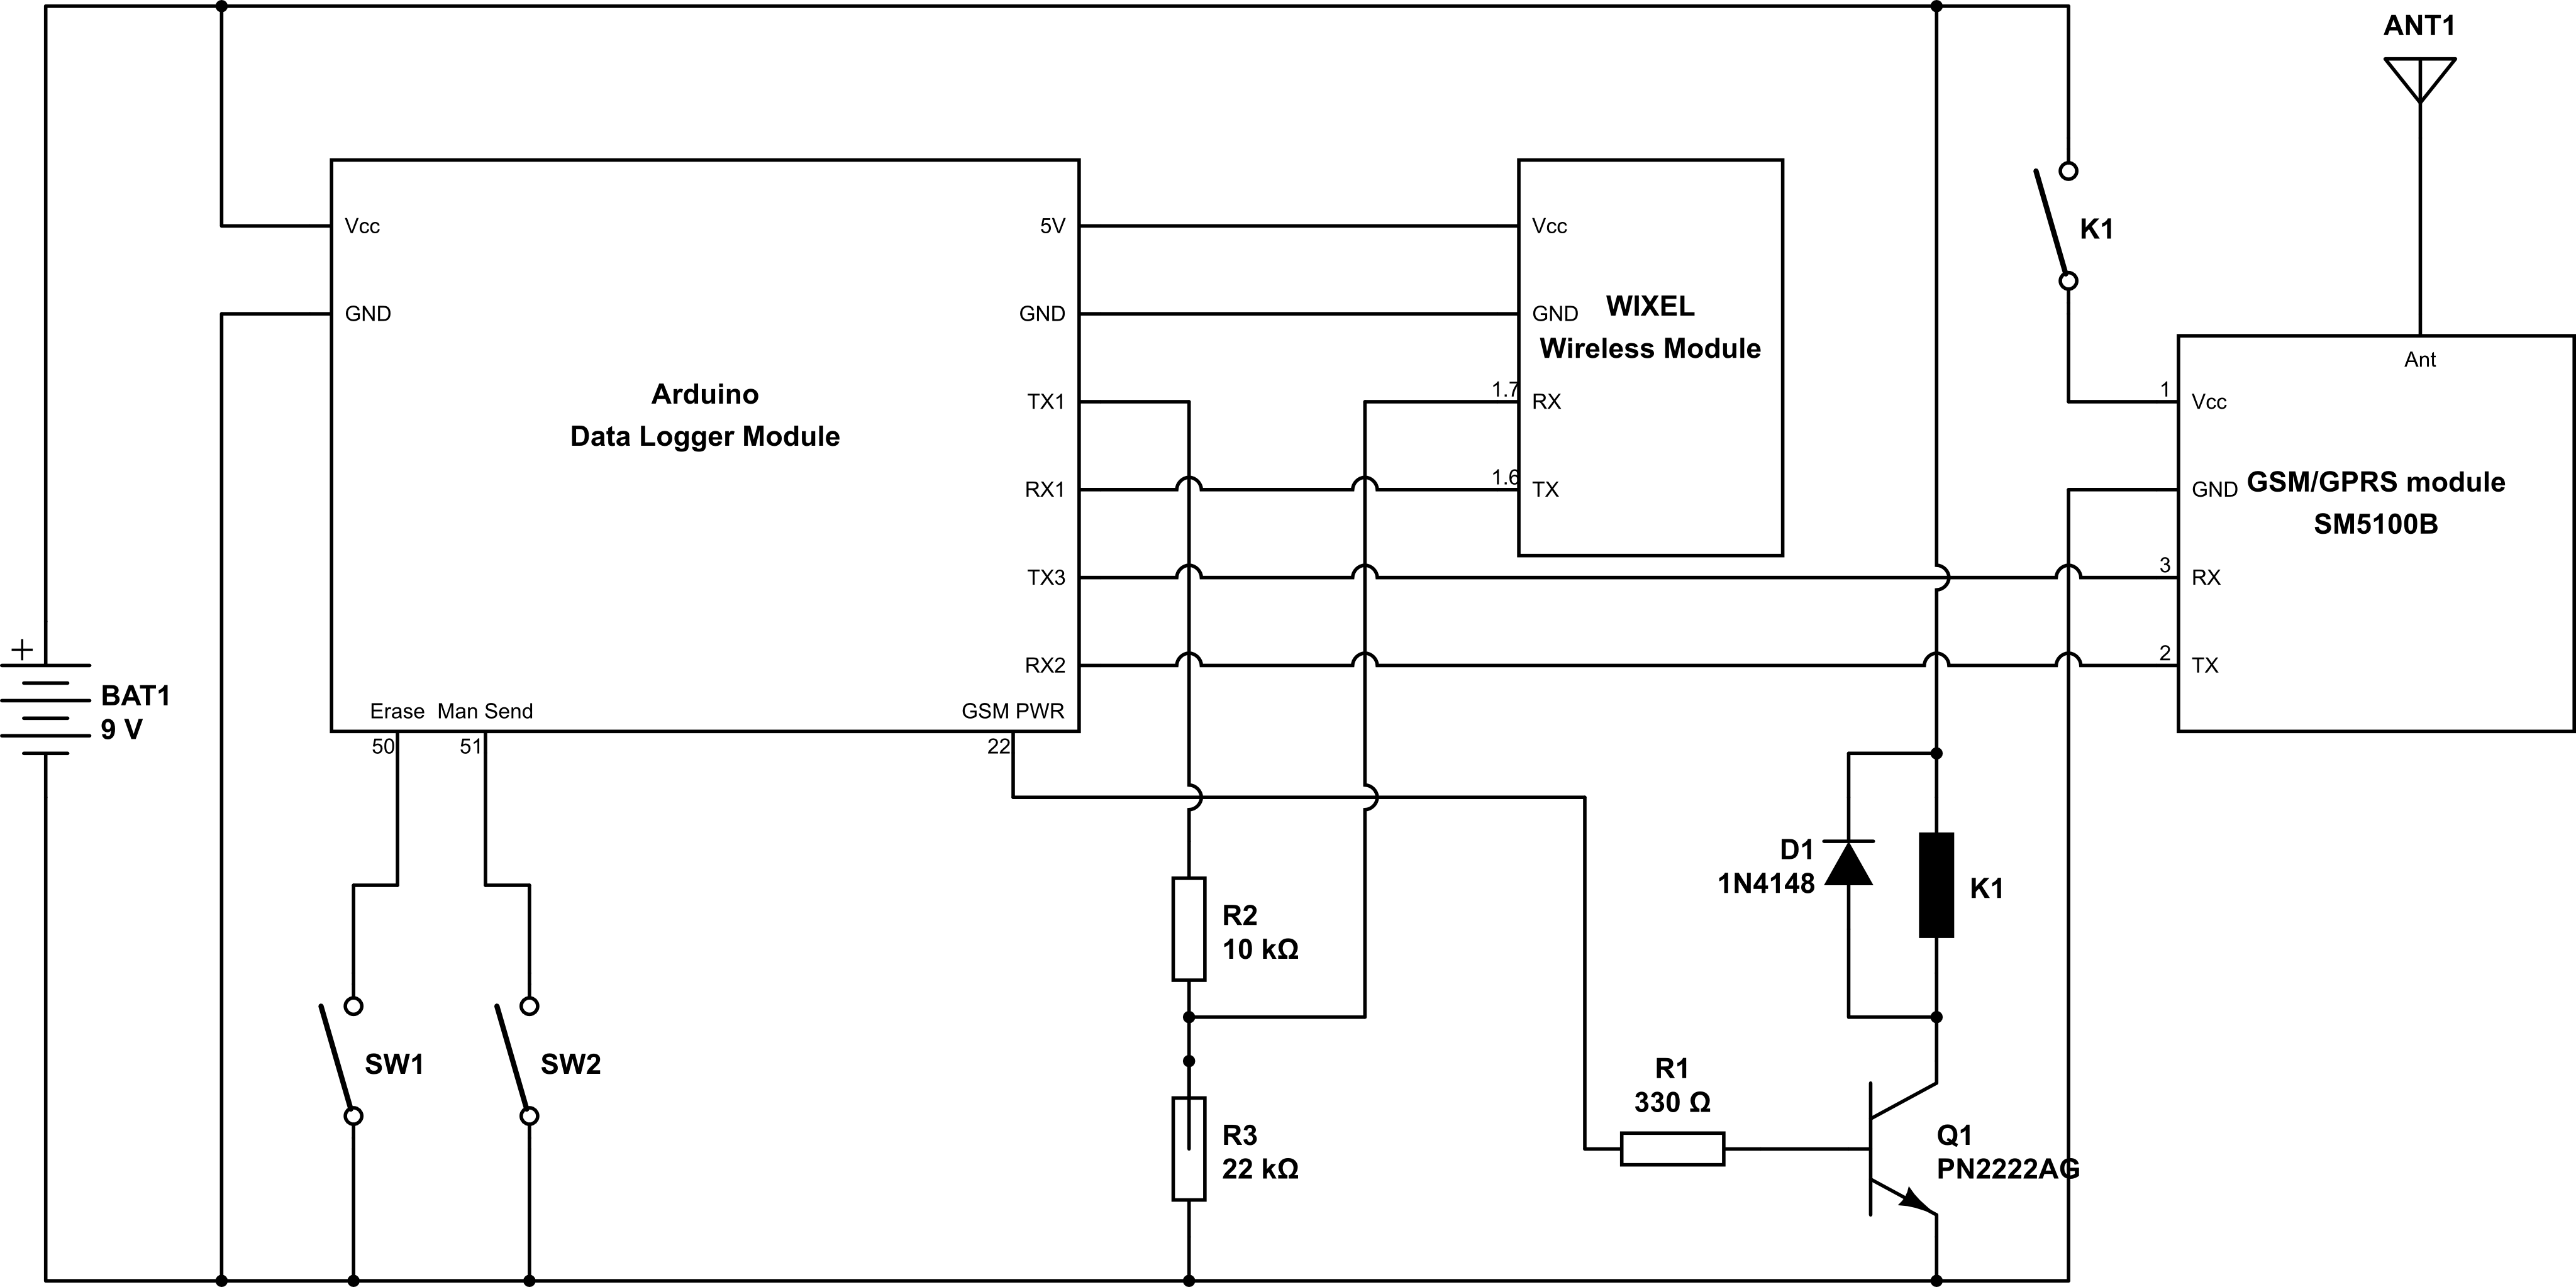
\includegraphics[width=1\linewidth]{graphics/motherhub_schematic}
\caption{Electrical Schematic Diagram of the Mother Hub\label{fig:motherhub_schematic}}
\end{figure}

\begin{figure}[H]
\centering
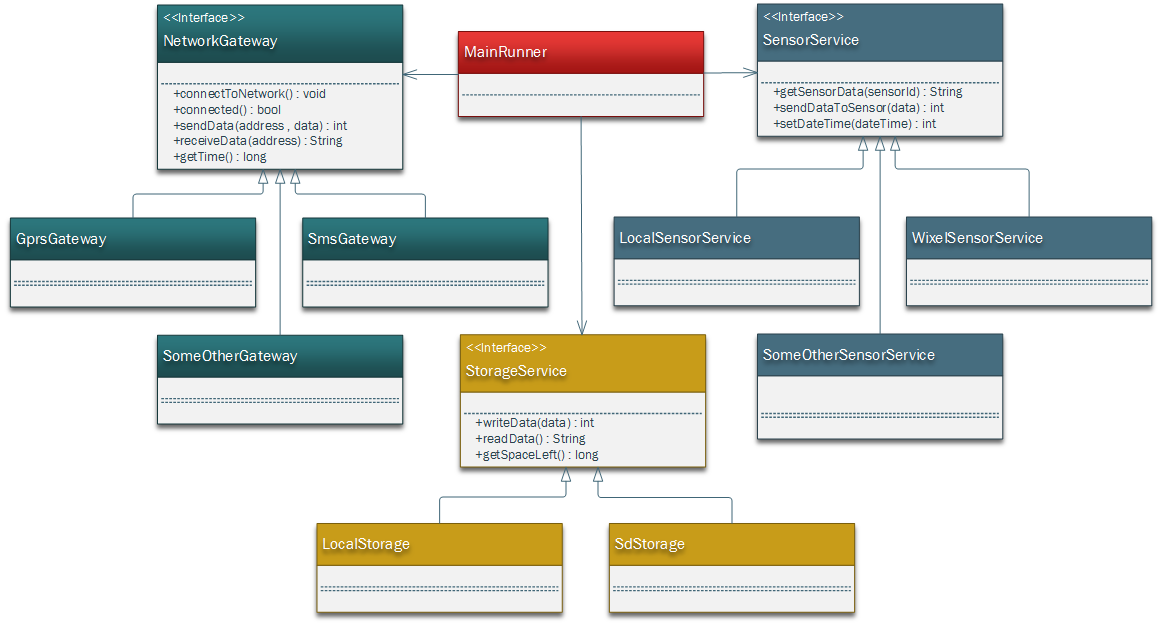
\includegraphics[width=1\linewidth]{graphics/ClassDiagram}
\caption{Class Diagram of the system\label{fig:ClassDiagram}}
\end{figure}

\addcontentsline{toc}{subsection}{HTTP Server}
\subsection*{HTTP Server}
\begin{lstlisting}[frame=single, label=httpCode, caption={Code for the HTTP server language=Python}]
import json, time
from flask import Flask, request
from flask.ext import restful
import datetime
from numpy import mean


class DataStorage(object):
    
    def __init__(self, file_name):
        self.file = file_name
    def append(self, dict):
        with open(self.file, 'a') as f:
            json.dump(dict, f)

    def get_data(self):
        try:
            with open(self.file) as f:
                json_array = ['{'+x+'}' for x in f.read().strip('{}').split('}{')]
                return [json.loads(x) for x in json_array]
        except:
            return []      


app = Flask(__name__)
api = restful.Api(app)
alldata = DataStorage('data.json')

@app.route('/geoblog')
def hello():
    dataGathered =  alldata.get_data()
    lastRecieved = ""
    site = '<!DOCTYPE html>' \
         + '<html class="full" lang="en">'\
         + '<head>'\
         + '<meta charset="utf-8">'\
         + '<title>GeoBlog</title>'\
         + '<link href="http://bootswatch.com/cosmo/bootstrap.min.css" rel="stylesheet">'\
         + '</head>'\
         + '<body>'\
         + '<div class="container"> <div class="jumbotron">'\
         + '<h1>GeoBlog</h1>' \
         + '<h3>Average Temperature: ' + str(mean([int(t['temp']) for t in dataGathered])) + '</h3>' \
         + '</div></div><div class="container">'

    for i in range(0, len(dataGathered)):
        
        if dataGathered[i]['received'] != lastRecieved:
            site += '<div class="panel panel-default">'\
                 + '<div class="panel-heading"> Received at: ' +dataGathered[i]['received'] + '</div>' \
                 + '<div class="panel-body">'\
                 + '<table class="table"><tr><th>Timestamp sek</th><th>Sensor Id</th><th>Temperature &degC</th></tr>'

        site += '<tr><td>' + str(int(dataGathered[i]['date'])/1000) + '</td>' \
              + '<td>' + dataGathered[i]['sensorId'] + '</td>' \
              + '<td>' + dataGathered[i]['temp'] + '</td></tr>'
        
        if i < len(dataGathered) - 1:
            if dataGathered[i + 1]['received'] != dataGathered[i]['received']:
                site += '</table></div></div>'

        lastRecieved = dataGathered[i]['received']
            
    site += '</div>'\
          + '</body>' \
          + '</html>' 
    return site
          #+ '<script src="js/jquery-1.10.2.js"></script>' \
          #+ '<script src="js/bootstrap.js"></script>' \


class ApiGeoLog(restful.Resource):
    def get(self):  
       return alldata.get_data()   

    def post(self):
        dataRecieved = request.data
        #print str(dataRecieved)
        data = json.loads(dataRecieved)
        for d in data:
            #print str(d)
            if d['date'] != None and d['temp'] != None and d['sensorId'] != None:
                d['received'] = datetime.datetime.now().strftime("%d. %B %Y %H:%M")
                alldata.append(d)
        
        return 'ok', 200


api.add_resource(ApiGeoLog, '/geolog')


if __name__ == '__main__':
    #app.debug = True    
    
    app.run(host='0.0.0.0', threaded=True)

\end{lstlisting}